% !TeX program = XeLaTeX or LuaLaTeX
% !TeX encoding = UTF-8 Unicode
% TEMPLATE.TEX
%
% Time-stamp: <2013-03-26 11:09 olenz>
% Update: Okt. 2020, Samuel Maier: Warnungen beseitigt, scrpage hinzugefügt, für online-PDF optimiert, konkret Verwendet.
%
% This is an extensively documented LaTeX file that shows how to
% produce a good-looking document with current LaTeX (11/2012).
%
% IMPORTANT!
%
%   Some obsolete commands and packages
% ----------|-------------------------------
% obsolete  |     Replacement in LATEX 2ε
% ----------|-------------------------------
%           | local            global/switch
% ----------|-------------------------------
% {\bf ...} | \textbf{...}     \bfseries
%     -     | \emph{...}       \em
% {\it ...} | \textit{...}     \itshape
%     -     | \textmd{...}     \mdseries
% {\rm ...} | \textrm{...}     \rmfamily
% {\sc ...} | \textsc{...}     \scshape
% {\sf ...} | \textsf{...}     \sffamily
% {\sl ...} | \textsl{...}     \slshape
% {\tt ...} | \texttt{...}     \ttfamily
%     -     | \textup{...}     \upshape
%
% DON'T USE \\ TO MAKE LINEBREAKS, INSTEAD JUST LEAVE A BLANK LINE!
%
\RequirePackage[l2tabu,orthodox]{nag} % turn on warnings because of bad style
\documentclass[a4paper,english,12pt,twoside=false]{scrartcl} %bibliography=totoc,
%
%%%%%%%%%%%%%%%%%%%%%%%%%%%%%%%%%%%%
% KOMA CLASSES
%%%%%%%%%%%%%%%%%%%%%%%%%%%%%%%%%%%%
%
% The class "scrartcl" is one of the so-called KOMA-classes, a set of
% very well done LaTeX-classes that produce a very European layout
% (e.g. titles with a sans-serif font).
% 
% The KOMA classes have extensive documentation that you can access
% via the commands:
%   texdoc scrguide # in German
%   texdoc scrguien # in English
%   
%
% The available classes are:
%
% scrartcl - for "articles", typically for up to ~20 pages, the
%            highest level sectioning command is \section
%
% scrreprt - for "reports", typically for up to ~200 pages, the
%            highest level sectioning command is \chapter
%
% scrbook  - for "books", for more than 200 pages, the highest level
%            sectioning command is \part.
%
% USEFUL OPTIONS
%
% a4paper  - Use a4 paper instead of the default american letter
%            format.
%
% german   - Use german default for packages, especially babel
%
% 11pt, 12pt, 10pt 
%          - Use a font with the given size.
%
% bibtotoc - Add the bibliography to the table of contents
%
% The KOMA-script classes have plenty of options to modify

% This allows to type UTF-8 characters like ä,ö,ü,ß
\usepackage{babel}

\usepackage[T1]{fontenc}        % Tries to use Postscript Type 1 Fonts for better rendering
\usepackage{lmodern}            % Provides the Latin Modern Font which offers more glyphs than the default Computer Modern
\usepackage[intlimits]{amsmath} % Provides all mathematical commands
\usepackage{amssymb}            % Provides amonst others the qed symbol
\usepackage{aligned-overset}    % allows for alignation of overset/underset chars by their main argument instead of the combined symbol
\usepackage{enumitem}			% allows to make listings with different enumerations, e.x. a,b,c

\usepackage{hyperref}           % Provides clickable links in the PDF-document for \ref
\usepackage{grffile}            % Allow you to include images (like graphicx). Usage: \includegraphics{path/to/file}

% Allows to set units
\usepackage[ugly]{units}        % Allows you to type units with correct spacing and font style. Usage: $\unit[100]{m}$ or $\unitfrac[100]{m}{s}$

% Additional packages
\usepackage{url}                % Lets you typeset urls. Usage: \url{http://...}
\usepackage{xspace}             % Use \xpsace in macros to automatically insert space based on context. Usage: \newcommand{\es}{ESPResSo\xspace}
\usepackage{xcolor}             % Obviously colors. Usage: \color{red} Red text
\usepackage{booktabs}           % Nice rules for tables. Usage \begin{tabular}\toprule ... \midrule ... \bottomrule

\usepackage{fontspec}
% Source code listings
\usepackage{listings}           % Source Code Listings. Usage: \begin{lstlisting}...\end{lstlisting}
%\usepackage{lstfiracode}

\usepackage{float}

%\setmonofont[Contextuals={Alternate}]{Fira Code Regular}
%\setsansfont{Calibri}

\restylefloat{table}

\definecolor{codegreen}{rgb}{0,0.6,0}
\definecolor{codegray}{rgb}{0.5,0.5,0.5}
\definecolor{codepurple}{rgb}{0.58,0,0.82}
\definecolor{backcolour}{rgb}{0.95,0.95,0.92}

\lstdefinestyle{mystyle}{
    backgroundcolor=\color{backcolour},
    commentstyle=\color{codegreen},
    keywordstyle=\color{magenta},
    basicstyle=\ttfamily\small,
    breaklines=true
    % frame=shadowbox,
%     numberstyle=\tiny\color{codegray},
%     stringstyle=\color{codepurple},
%     basicstyle=\footnotesize,
%     breakatwhitespace=false,
%     breaklines=true,
%     captionpos=b,
%     keepspaces=true,
%     % numbers=left,
%     % numbersep=5pt,
%     showspaces=false,
%     showstringspaces=false,
%     showtabs=false,
%     tabsize=2
}

\lstset{style=mystyle}

% Add the ability to actually set the header and footer
\usepackage[footsepline=true]{scrlayer-scrpage}
\pagestyle{scrheadings}


\begin{document}

\sffamily % Use sans-serif font (I hate serif-fonts)

\newcommand{\module}{HPC\xspace}
\newcommand{\group}{Gruppe GjeSam, WS 21/22\xspace}
\newcommand{\breakln}{\mbox{} \\}

\titlehead{High Performance Computing Wintersemester 21/22, HFT Stuttgart \hfill WS 2021/2022}
\title{Abschlussprojekt}
\author{
  \textbf{\group:} \\
  Gjergji Shkurti, 357059\\
  Samuel Maier, 1002330
}
\date{\today}

\lohead{\group}
\cohead{Abschlussprojekt}
\rohead{\module, HFT Stuttgart}

\maketitle

\pagebreak

\tableofcontents

\pagebreak

\section{Motivation}

The purpose of this project is to solidify the knowledge gained in this course.

As such we decided to choose a simple suggestion as basis for our Project, this allows us to dive deeper into the topic without distractions, and this particular issue can be extended if neccessary.

That is also the reason we decided to minimize the UI. We also decided to default to headless running by default, as the input and output of the result would probably be the major limiting factor in most optimizations.

A major extension we waned to look at, if we get to it, was to use our headless running game to detect cycles in the loop.

\section{Problem statement}

Our Issue started out as a naive \verb|C++| Implementation.


\footnote{TODO}

% TODO

\pagebreak

\section{Game Of Life Implementation}

\subsection{Rules of the Game}

The Game of Life, also known simply as Life, is a cellular automaton devised by the British mathematician John Horton Conway in 1970. It is a zero-player game, meaning that its evolution is determined by its initial state, requiring no further input. One interacts with the Game of Life by creating an initial configuration and observing how it evolves.

\breakln

Rules of the game:

\begin{itemize}
	\item{Any live cell with fewer than two live neighbours dies, as if by underpopulation}
	\item{Any live cell with two or three live neighbours lives on to the next generation}
	\item{Any live cell with more than three live neighbours dies, as if by overpopulation}
	\item{Any dead cell with exactly three live neighbours becomes a live cell, as if by reproduction}
\end{itemize}

These rules, which compare the behavior of the automaton to real life, can be condensed into the following:

\begin{itemize}
	\item{Any live cell with two or three live neighbours survives}
	\item{Any dead cell with three live neighbours becomes a live cell}
	\item{All other live cells die in the next generation. Similarly, all other dead cells stay dead}
\end{itemize}

\subsection{Naive Implementation}

For the naive implementation of Game of Life, the data structure depicted at listing \ref{lst:gol-naive-board-datastructure} is used to represent the board-relevant data. The board consists of a multi-dimensional vector of size \textbf{row{\_}nr x col{\_}nr}  containing integers which represent the cells themselves. Each cell can have a value of 0 (dead) or 1 (alive).

\begin{lstlisting}[caption={Game of Life Board Datastructure},label={lst:gol-naive-board-datastructure},language=C++]
typedef struct
{
    std::vector<std::vector<int>> cell_rows;
    int row_nr;
    int col_nr;
} board_t;.
\end{lstlisting}

To test the performance of the implementation in a reproducable way, the initial state of the board is initialized with a glider pattern\footnote{placeholder} on the top left corner of the board. During the execution, a configurable amount of world states\footnote{placeholder} is generated. Each state can be displayed using a simplistic console based GUI. The displaying of the states is however deactivated and not taken into account when measuring the performance of the implementation as it would be the major performance limiting factor. \newline

A naive way of solving the state generation problem is to loop through each cell of the board and calculate the living neighbour count of the cell. (see listing \ref{lst:gol-naive-neighbour-counting}). Then, calculate the next cell state for each cell by taking into account the previously calculated living neighbour count and applying the rules of the game accordingly. 

\begin{lstlisting}[caption={Naive Neighbour Counting},label={lst:gol-naive-neighbour-counting},language=C++]

// Get the neighbour count of the cell at (row:col) of the board
int get_neighbour_count(int row, int col, board_t& board) {
    int neighbour_count = 0;
    int indexes[3] = { -1, 0, 1 };
    // Check col
    for (int i : indexes) {
        // Check Row
        for (int j : indexes) {
            // Avoid the current cell
            if (j || i) {
                // Add cell state (0|1) to neighbour count
                neighbour_count += cell_state_at(row + j, col + i, board);
            }
        }
    }
    return neighbour_count;
}

\end{lstlisting}

Note that it is important to make a copy of the current board state and calculate the next state for each cell by taking the copy board into account. Otherwise the current state would get corrupted during the application of the rules by the algorithm. A C++ implementation of the state generation algorithm can be seen in listing \ref{lst:gol-naive-generation-algorithm}.

\begin{lstlisting}[caption={Naive State Generation Algorithm},label={lst:gol-naive-generation-algorithm},language=C++]

int generate_cell_state(int row, int col, board_t& board){
    int cell_neighbour_count = get_neighbour_count(row, col, board);
    int cell_survives = board.cell_rows.at(row).at(col) && (cell_neighbour_count == 2 || cell_neighbour_count == 3);
    int cell_birth = !board.cell_rows.at(row).at(col) && (cell_neighbour_count == 3);
    return cell_survives || cell_birth;
}

void generate_next_board_state(board_t& current_board_state) {
    //Store current board state to avoid overriding during cell state generation
    board_t temp = current_board_state;
    // Loop through rows
    for (int row = 0; row < current_board_state.row_nr; row++) {
        // Loop through cols
        for (int col = 0; col < current_board_state.col_nr; col++) {
        	//Generate cell State
        		current_board_state.cell_rows.at(row).at(col) = generate_cell_state(row, col, temp);
        }
    }
}
\end{lstlisting}

\subsubsection{OpenMP Parallelization}

\begin{table}
\centering
\begin{tabular}{|l|l|l|l|l|l|} 
\hline
\begin{tabular}[c]{@{}l@{}}Board \\Size\end{tabular} & \begin{tabular}[c]{@{}l@{}}Serial\\Speed (ms)\end{tabular} & \begin{tabular}[c]{@{}l@{}}OpenMP\\Speed (ms)\end{tabular} & \begin{tabular}[c]{@{}l@{}}Relative\\Speedup\end{tabular} & \begin{tabular}[c]{@{}l@{}}Cache Misses\\Serial\end{tabular} & \begin{tabular}[c]{@{}l@{}}Cache Misses\\OpenMP\end{tabular} \\ 
\hline
10x10 & 206 & 188 & 1,09 & 80.053 & 105.237 \\ 
\hline
16x16 & 447 & 394 & 1,13 & 90.192 & 129.299 \\ 
\hline
32x32 & 1625 & 648 & 2,50 & 194.906 & 213.505 \\ 
\hline
64x64 & 6287 & 1921 & 3,27 & 400.519 & 421.363 \\ 
\hline
128x128 & 24501 & 7416 & 3,30 & 996.068 & 1.450.321 \\ 
\hline
256x256 & 104478 & 32401 & 3,22 & 4.546.139 & 5.557.419 \\
\hline
\end{tabular}
\caption{OpenMP Performance Comparison}
\label{tab:naive-performance-metrics}
\end{table}

The main benefit of the naive implementation of Game of Life is that it is fairly easy to parallelize as computing the value of a cell in the current generation does not depend on the computations of the neighbouring cells. Each thread is only responsible for reading the data of a particular board area. All parallel threads read the current board state from the copy of the board mentioned above but none of them write in the same block of the array. This means that there is no need for synchronization between the threads and therefore no performance hits are incurred due to synchronization related overhead. Thus, OpenMP can be used to easily parallelize the naive state generation algorithm as seen in listing \ref{lst:gol-parallel-naive-generation-algorithm}. The only critical part is the updating of current the board state which can be done by a single thread to avoid the need for synchronization. Table \ref{tab:naive-performance-metrics} provides an overview of the performance difference between the serial and parallel implementations (8 threads) of the naive algorithm with different board sizes on an 8 core Intel(R) Core(TM) i7-10510U CPU @ 1.80GHz processor.

\begin{lstlisting}[caption={Parallel Naive State Generation Algorithm},label={lst:gol-parallel-naive-generation-algorithm},language=C++]
void game_of_life_loop_omp(board_t& board, board_t& temp, int generations, int display)
{
#pragma omp parallel num_threads(12)
    {
        num_threads = omp_get_num_threads();
        for (int gen = 0; gen < generations; gen++) {
#pragma omp for
            for (int row = 0; row < board.row_nr; row++) {
                for (int col = 0; col < board.col_nr; col++) {
                    int alive_neighbours = get_neighbour_count(row, col, board);
                    int cell_survives = board.cell_rows.at(row).at(col) && (alive_neighbours == 2 || alive_neighbours == 3);
                    int cell_birth = !board.cell_rows.at(row).at(col) && (alive_neighbours == 3);
                    temp.cell_rows.at(row).at(col) = cell_survives || cell_birth;
                }
            }
#pragma omp master
            {
                board.cell_rows.swap(temp.cell_rows);

                if (display) {
                    display_board_state(board);
                }
            }
#pragma omp barrier
        }
    }
}
\end{lstlisting}

\subsubsection{Limiting Factors - Cache Performance}

One limiting factor of the naive implementation is the rather poor cache performance. In Linux, cache misses can be measured by using the perf tool\footnote{placeholder} (sudo perf stat -e cache-misses <executable>). Table \ref{tab:naive-performance-metrics} provides an overview of the cache misses incurred when running 100000 iterations of the naive Game of Life algorithm with different board sizes.

\subsubsection{Limiting Factors - Memory Bottleneck}

When analyzing the performance of the naive implementation using the Roofline Model\footnote{placeholder}, it becomes apparent that the implementation is primarily memory bound. A lot of time is spent allocating vectors (see blue boxes in figure \ref{fig:roofline-naive-32-100k}) when making a copy of the current board state in $generate{\_}next{\_}board{\_}state{\_}(board{\_}t{\&}{\ }board)$. The compute intensity of this method as well as the method for getting the neighbour count is very low. One can also see that the largest bottleneck of the algorithm itself is the $cell{\_}state{\_}at(int{\ }row,{\ }int{\ }col,{\ }board{\_}t{\&}{\ } board)$ (1st red box in figure \ref{fig:roofline-naive-32-100k} method which is reponsible for looking up the eight neighbouring cells of the selected cell. This particular way of looking up the neighbouring cells in the two dimensional vector is very cache inefficient as evidenced by the cache misses discussed in the previous subsection of this document. As we are memory bound and not compute bound, the benefit of parallelizing the algorithm is greatly reduced as is evidenced by the fact that the speedup factor depicted in table \ref{tab:naive-performance-metrics} plateaus after increasing the board size from 64x64 to 128x128. 

\begin{figure}[tbh!]
	\centering
	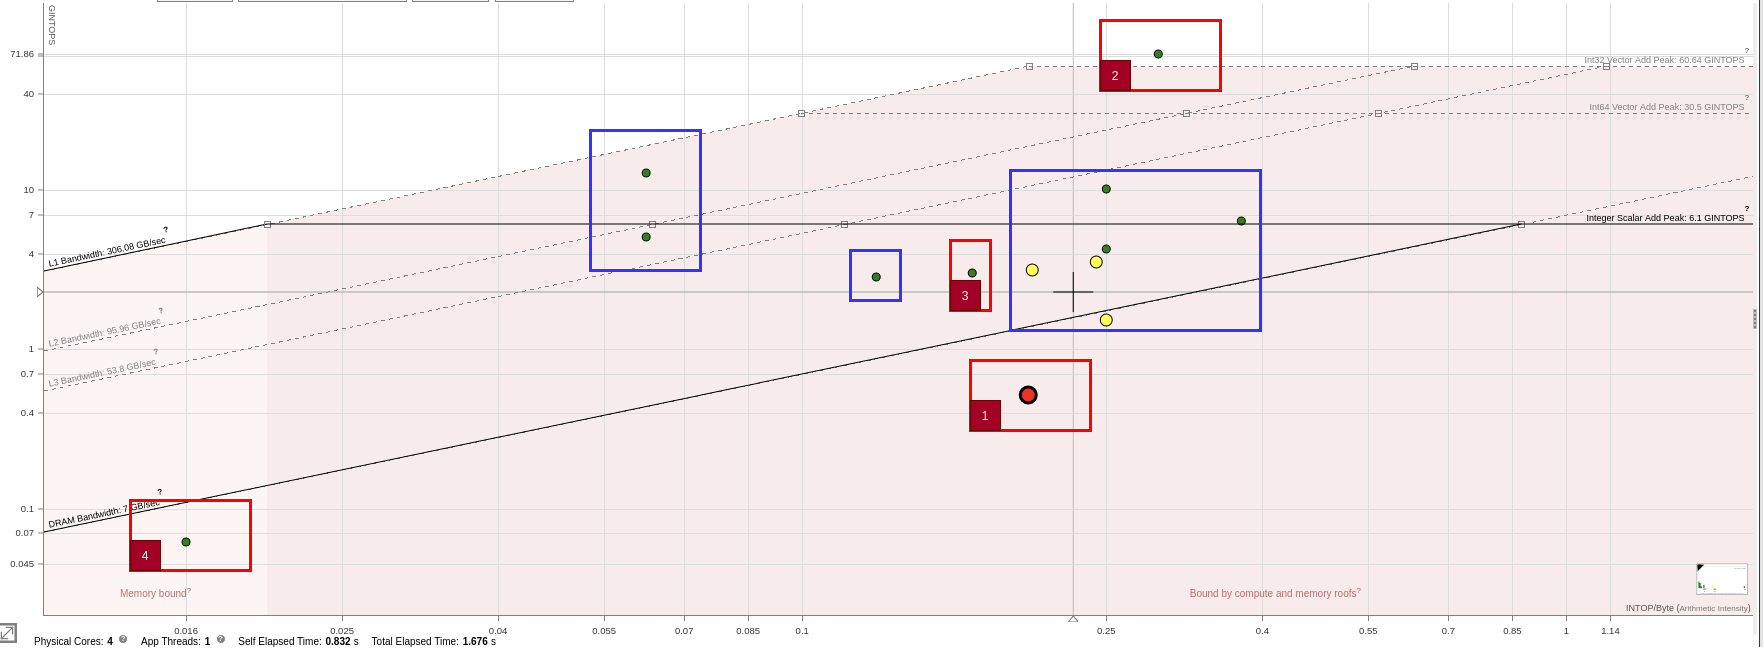
\includegraphics[width=16cm]{imgs/roofline-naive-32-100k.png}
	\caption{Roofline Analysis Results - Naive - Serial}
	\label{fig:roofline-naive-32-100k}
\end{figure}

\subsection{Optimized Implementation}

As previously mentioned, the naive algorithm is easy to parallelize and therefore suitable for a framework such as OpenMP. However, the algorithm itself is rather inefficient in regards to memory and cache optimizations and as such can only benefit so much from being parallelized. In this chapter, an optimized version of the algorithm and a better way of representing the cell-relevant data to increase cache performance are discussed.

\subsubsection{Optimized Data Representation}

Another approach to solving the state generation problem is to encode both the cell state and the number of living neighbours a cell has into a single data structure. Then, when manipulating the state of a cell, one can accordingly increment or decrement the number of living neighbours for each of the surrounding cell. Lets consider cell-relevant data. A cell has a state (dead/alive) which can be encoded into a single bit (1/0). It can have a minimum of 0 living neighbours and a maximum of 8, which can be represented by using only 4 bits. So, to store all relevant cell data, we need a total of 5 bits. We can store all cell-relevant data in the first 5 bits of an unsigned char\footnote{placeholder} (see figure \ref{fig:cell-state}). Keeping this in mind, we can store the state of all cells of the board into a one dimensional array of unsigned chars. By using a smaller datatype, we greatly reduce the ammount of memory needed to store our board states compared to the previous naive implementation. The other benefits of representing our data in this way are discussed in the following subsection of this document. Listing \ref{lst:gol-optimized-datastructure} depicts the optimized structure of storing all board-relevant data.

\begin{lstlisting}[caption={Parallel Naive State Generation Algorithm},label={lst:gol-optimized-datastructure},language=C++]

typedef struct
{
    u_char* cells = nullptr;
    u_int rows;
    u_int cols;
    u_int length;
} board_t;

\end{lstlisting}

\begin{figure}[tbh!]
	\centering
	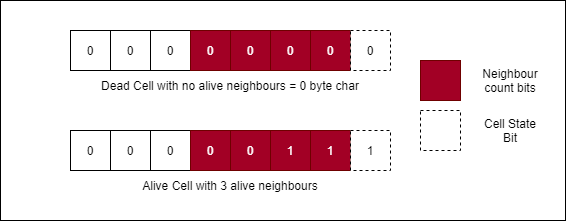
\includegraphics[width=16cm]{imgs/cell-state.png}
	\caption{Cell State Char}
	\label{fig:cell-state}
\end{figure}

\subsubsection{Optimized Board State Generation Algorithm}

\begin{figure}[tbh!]
	\centering
	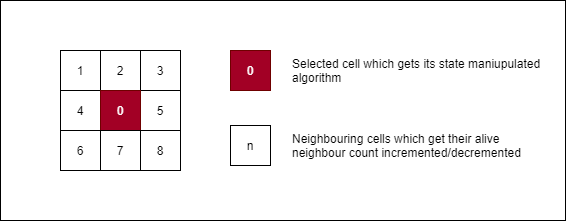
\includegraphics[width=16cm]{imgs/cell-algo.png}
	\caption{Optimized Generation Algorithm}
	\label{fig:cell-algo}
\end{figure}

As shown in figure \ref{fig:cell-state}, a dead cell with no alive neighbours is simply a 0 byte. These cells can never change their state. We can skip applying the rules of the game to all cells that fulfill the requirement of being 0 bytes. This has two benefits: Firstly, our algorithm gains a significant performance increase as it can simply access the cell via a pointer and check whether the dereferenced value of the pointer is 0. If that is the case, it can skip analyzing the cell and move on to its neighbour. Secondly, the overall state of the game of life tends towards a sparse state. This means, on a randomly initialized board, the further we are in our iterations, the larger the number of dead cells without any living neighbours is. Because our algorithm simply such cells, its performance gain becomes larger the further we are in our iterations.


Listing \ref{lst:gol-optimized-manipulation} depicts the method for setting the cell of a state to dead and deincrementing the neighbour counts of its surrounding neighbours. Bitwise manipulation is used to set the intial bit of the unsigned char representing the cell data to 0. Then, bitwise manipulation is used to remove one to the neighbour count of each of the cells 8 neighbours. Setting the cell state to alive is similar. The only difference is that the first bit is set to 1 ($*(cell_ptr) |= 0x01$)  and the count of each neighbour is incremented by one ($*(cell_ptr + y + x) += 0x02$).

\begin{lstlisting}[caption={Parallel Naive State Generation Algorithm},label={lst:gol-optimized-manipulation},language=C++]

// "Kill" the cell by setting its first bit to 0 and deincrement all of its 8 neighbours living cell counts by one
void kill_cell(board_t& board, const u_int& row, const u_int& col) {
    // index 1d array as 2d array
    u_char* cell_ptr = board.cells + (col * board.cols) + row;
     // kill the cell by setting first bit to 0
    *(cell_ptr) &= ~0x01;
    // Handle indexes if the cell is on the edges of the board
    int x_left, x_right, y_above, y_below;
    get_wrap_indexes(board, row, col, x_left, x_right, y_above, y_below);
    // Deincrement the neighbour count of all surrounding cells since the cell died
    *(cell_ptr + y_above + x_left) -= 0x02;
    *(cell_ptr + y_above) -= 0x02;
    *(cell_ptr + y_above + x_right) -= 0x02;
    *(cell_ptr + x_left) -= 0x02;
    *(cell_ptr + x_right) -= 0x02;
    *(cell_ptr + y_below + x_left) -= 0x02;
    *(cell_ptr + y_below) -= 0x02;
    *(cell_ptr + y_below + x_right) -= 0x02;
}
\end{lstlisting}

Listing \ref{lst:gol-optimized-algo} depitcs the optimized state generation algorithm. As previously discussed, we initially check if the selected cell is a 0 byte and if that is the case, we skip the application of the rules. If the requirement for skipping is not fulfilled, the alive neighbour count of the cell is acquired by using a bitwise shift operation on the unsigned char representing the cell-relevant data. If the data of the unsigned char is shifted by one to the right, the state bit becomes a carry bit. Therefore, the only remaining data in the unsigned char are the 4 bits representing the alive neighbour count of the selected cell. Depending on this number, we apply the rules of the game to the cell and update all neighbouring cells accordingly.

\begin{lstlisting}[caption={Parallel Naive State Generation Algorithm},label={lst:gol-optimized-algo},language=C++]
void generate_next_board_state(board_t& board, board_t& temp_board) {
    memcpy(temp_board.cells, board.cells, board.length);

    for (u_int index = 0; index < board.rows * board.cols; index++) {
        auto lookup_cell_ptr = temp_board.cells + index;
        if (*lookup_cell_ptr == 0)
            continue;
        auto nb_count = (*lookup_cell_ptr) >> 1;
        bool is_alive = (*lookup_cell_ptr) & 0b01;

        if (is_alive) {
            // if the cell stays alive, skip
            if (2 <= nb_count && nb_count <= 3)
                continue;
            u_int col = index % board.rows;
            u_int row = index / board.rows;
            // // kill the cell
            kill_cell(board, col, row);
        } else {
            // cell only gains life when it has precisely 3 neighbours
            if (nb_count != 3)
                continue;
            u_int col = index % board.rows;
            u_int row = index / board.rows;
            spawn_cell(board, col, row);
        }
    }
}
\end{lstlisting}

Note that the cache performance of this implementation, tested on a board containing a single glider, is much better than the previous naive implementation. (see table \ref{tab:optimized-cache-misses}). Despite the fact that the implementation is not parallelized, the optimized state generation algorithm performs much better than the naive implementation, particularly on smaller board sizes. 

\begin{table}
\centering
\begin{tabular}{|l|l|l|l|} 
\hline
\begin{tabular}[c]{@{}l@{}}Board \\Width\end{tabular} & \begin{tabular}[c]{@{}l@{}}Speed~\\(ms)\end{tabular} & \begin{tabular}[c]{@{}l@{}}Cache\\Misses\end{tabular} & \begin{tabular}[c]{@{}l@{}}Speedup relative \\to the OpenMP \\Naive Implementation\end{tabular} \\ 
\hline
10x10 & 10 & 57.109 & 18,8 \\ 
\hline
16x16 & 21 & 76.464 & 18,76 \\ 
\hline
32x32 & 68 & 89.584 & 9,52 \\ 
\hline
64x64 & 253 & 84.346 & 7,59 \\ 
\hline
128x128 & 1044 & 108.983 & 7,10 \\ 
\hline
256x256 & 4273 & 206.050 & 7.58 \\
\hline
\end{tabular}
\caption{Performance - Optimized}
\label{tab:optimized-cache-misses}
\end{table}


\subsubsection{Difficulty with parallelizing the optimized Algorithm}

TODO!!!

\subsection{OpenCL Implementation}

To use OpenCL at all we had to do qite a bit of work, since we had a Makefile based build process, so we had build the Application using mostly \verb|wsl|, but passing a GPU to \verb|wsl| is no small feat. So we installed a native Linux OS.

We were also triggered to rethink the implementation fundamentally for OpenCL, since it has more explicit memory tiers than executions on the CPU with implicit caching.

OpenCL prefers to group parts of the algorithm in 2 levels, one individual problem - \verb|Work-Item|s - and a group of them together - \verb|Work-Group|. Items in a group can coordinate with shared memory, and access to that memory is usually a magnitude faster than access to global memory, that is shared by all Groups (so shared among the entire algorithm).

We want to utilize this of course. But another problem is the execution and branching. All work-items in a work-group must be assumed to be executed together with one instruction pointer.

This means that for starters the slowest work-item will determine the combined execution speed. But the coupling is stronger than that. If the code includes branching, AND both branches get executed, these branches must be executed AFTER one another, because of the single instuction pointer per work-group (in reality these assumtions are not always true, but work-items and groups are meant to be abstractions on vendor-specific architectures, that usually behave similar).

\subsubsection{Memory locality and branching}



\begin{center}
    \captionof{figure}{Memory-access pattern with work-groups}
    \label{fig:cl-mem-access}
    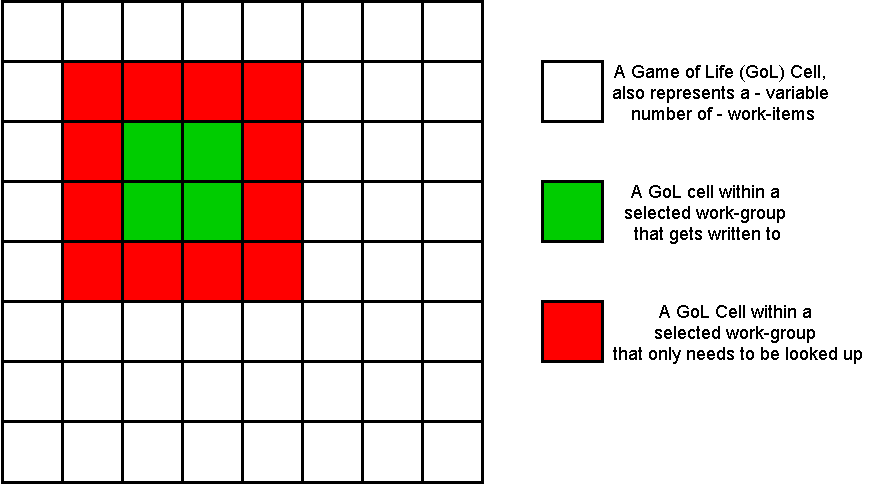
\includegraphics[width=\linewidth]{imgs/opencl_mem_access.pdf}
\end{center}

\section{Summary and conclusions}

\section{Appendix}

\begin{center}
    \captionof{figure}{Beispiel-Sourcecode}
    \label{fig:GameOfLife.cpp}
    \lstinputlisting[language=C++]{../src/common/Timing.cpp}
\end{center}

\end{document}